%\documentclass[twocolumn]{article}
\documentclass[./chem_exercises.tex]{subfiles}
\begin{document}

%\begin{titlepage}
%\maketitle
%\end{titlepage}


%\layout

%\chapter{Syntes av Koppar(II)sulfat}
\section{Framställan av diammoniumkoppar(II)sulfat hexahydrat}
Utrustning:\\
\begin{enumerate}
\item 1 st märkpenna
\item 1 st filter papper för att lägga kopparn vid vägning
\item 1 st 100 ml bägare med 12.5 ml markerad
\item 1 st mätkolv med avjoniserat vatten 15 ml därefter fylls 10 ml på
\item 1 st mätkolv med 2ml Salpetersyra
\item 1 st mätkolv med 4ml Svavelsyra
\item 1 st glasstav för omrörning
\item 1 st tratt med filter för gravitationsfiltrering
\item 1 st bägare för uppsamling av \ch{Cu(II)SO4}
\item 1 st Buchnertratt med tillbehör för sugfiltrering
\item 1 st en 100 ml bägare som i förväg markerats med
märkpenna för volymen 20 ml
\item Bägare med 6.3 ml 5M Ammoniak såsom uträknat
\item Bägare med 12.6 ml  2.5 M Svavelsyra såsom uträknat från balansekvationen
\item Koksten till Ammoniumsulfat framstälning
\item 1 st 100ml bägare som markerats i förväg till 20ml och innehållandes 20ml avjoniserat vatten
\item Koksten till diammoniumkoppar(II)sulfat-lösningen
\item Mätcylinder med 10 ml kall etanol



\end{enumerate}
\subsection{Substansmängder tillverknign Kopparsulfat}
\begin{enumerate}[label=(\alph*)]
\item Kopparpulver med massan 2g är i formen \ch{Cu(I)2O} och är ljusrött till färgen.
Molarmassan  $M_{\ch{Cu(I)2O}}$ är
\begin{flalign*}
M_{\ch{Cu(I)2O}}&= 2\cdot 63.546+15.9994 =143.09 \text{[g]}\cdot\text{[mol]}^{-1}
\end{flalign*} 

Substansmängden $n_{\ch{Cu(I)2O}}$ är\leavevmode\marginpar{$n_{\ch{Cu(I)2O}}= 0.013977\text{[mol]}$}
\begin{flalign*}
n_{\ch{Cu(I)2O}}&=\frac{m_{\ch{Cu(I)2O}}\text{ [g]}}{M_{\ch{Cu(I)2O}}\text{ [g]}\cdot\text{[mol]}^{-1}}\\
                &=\frac{2}{143.09}= 0.013977\text{ mol}
\end{flalign*} 
Om rent koppar avses så motsvara 2  gram \ch{Cu} substansmängden \leavevmode\marginpar{$n_{\ch{Cu}}= 0.031473\text{[mol]}$}
\begin{flalign*}
n_{\ch{Cu}}&=\frac{m_{\ch{Cu}}\text{ [g]}}{M_{\ch{Cu}}\text{ [g]}\cdot\text{[mol]}^{-1}}\\
                &=\frac{2}{63.546}= 0.031473\text{ mol}
\end{flalign*} 

\item 2.5M Koncentrerad Svalelsyra med volymen $4\text{ml}=0.004\text{dm}^3$ används,
vilken har substansmängden\leavevmode\marginpar{$n_{\ch{H2SO4}}= 0.010\text{[mol]}$}
\begin{flalign*}
n_{\ch{H2SO4}}&=c_{\ch{H2SO4}}[\text{mol}\cdot\text{dm}^{-3}]\cdot V_{\ch{H2SO4}}[\text{dm}^{3}]\\
              &=2.5\cdot0.004=0.010[\text{mol}]
\end{flalign*}

\item Koncentrerad 15M Salpetersyra med volymen $2\text{ml}=0.002\text{dm}^3$ används,
vilken har substansmängden\leavevmode\marginpar{$n_{\ch{HNO3}}= 0.030\text{[mol]}$}
\begin{flalign*}
n_{\ch{HNO3}}&=c_{\ch{HNO3}}[\text{mol}\cdot\text{dm}^{-3}]\cdot V_{\ch{HNO3}}[\text{dm}^{3}]\\
              &=15\cdot0.002=0.030[\text{mol}]
\end{flalign*}
Efter att man blandat kopparn med Salpetersyran och Svavelsyran under omrörning och reaktionen
avstannat så skulle man tillsätta ytteliggare $1ml$ Salpetersyra.\leavevmode\marginpar{$1 \text{ml }\ch{HNO3} \text{ är } 15\text{[mmol]}$}

\item Vatten med volymen $15\text{ml}=0.015\text{dm}^3$ används, vilken har 
molmassan $M_{\ch{H2O}}$
\begin{flalign*}
M_{\ch{H2O}}&=2\cdot1.00794+15.9994=18.015\text{[g]}\cdot\text{[mol]}^{-1}
\end{flalign*}
Antar att densiteten $\rho_{\ch{H2O}}=1\text{[g]}\cdot\text{[ml]}^{-1}$, så substansmängden
$n_{\ch{H2O}}$ är\leavevmode\marginpar{$n_{\ch{H2O}}= 0.8310\text{[mol]}$}
\begin{flalign*}
n_{\ch{H2O}}&=\frac{m_{\ch{H2O}}\text{ [g]}}{M_{\ch{H2O}}\text{ [g]}\cdot\text{[mol]}^{-1}}\\
                &=\frac{15}{18.015}= 0.8310\text{ mol}
\end{flalign*} 
\end{enumerate}

\subsection{Reaktionsformel Koppar och Salpetersyra}
Söker på internet och hittar att ren koppar reagerar med utspädd salpetersyra enligt
\begin{flalign*}
\ch{Cu}(s)+8\ch{HNO3}\rightarrow 3\ch{Cu(II)(NO3)2}+2\ch{NO}+4\ch{H2O}\\
\end{flalign*}
och med koncentrerad salpetersyra bildas istället rödfärgad \ch{NO2}
\begin{flalign*}
\ch{Cu}(s)+4\ch{HNO3}\rightarrow \ch{Cu(II)(NO3)2}+2\ch{NO2}(g)+2\ch{H2O}\\
\end{flalign*}

\subsection{Reaktionsformel Kopparnitrat och Svavelsyra}
Blanda i svavelsyra
\begin{flalign*}
\ch{Cu(II)(NO3)2}+\ch{H2SO4}&\rightarrow \ch{Cu(II)SO4}+\ch{H2}(g)+\ch{NO3^-}\\
\ch{NO3^-}(aq)+\ch{H2O}&\rightarrow \ch{HNO3} + \ch{OH^-}\\
\end{flalign*}


\subsection{Reaktionsformel Ammoniak och Svavelsyra}
\begin{flalign*}
\ch{NH3}+2\ch{H2SO4} \rightarrow \ch{(NH4)2SO4}
\end{flalign*}

\subsection{Substansmängder syntes ammoniumsulfat \ch{(NH4)2SO4}}
Uppgiften var att mäta upp lika stor mängd 5M Ammoniak som den substansmängd
koppar som mättes upp för att tillverka koppar(II)sulfat.
Eftersom rent koppar har accepterats som det som skall användas och inte Di-koppar(I)Oxid
så beräknas volymen för 0.031473 mol.\leavevmode\marginpar{$V_{NH3}(5M)\approx 6.3\text{ml}$}
\begin{flalign*}
n_{NH3}&=n_{\ch{Cu}}=0.031473\text{ mol}\\
V_{NH3}&=\frac{n_{NH3}\text{ mol}}{c_{NH3}\text{ mol}\cdot\text{dm}^{-3}}\\
       &=\frac{0.031473}{5}=6.2946e-03\text{dm}^3\approx 6.3 \text{ml}
\end{flalign*}
Vi har tillgång till Svavelsyra 2.5 M och behöver således lika stor substansmängd
\leavevmode\marginpar{$V_{H2SO4}(2.5M)\approx 6.3\text{ml}$}
\begin{flalign*}
n_{H2SO4}&=n_{n_{NH3}}=0.031473\text{ mol}\\
V_{H2SO4}&=\frac{n_{H2SO4\text{ mol}}}{c_{H2SO4}\text{ mol}\cdot\text{dm}^{-3}}\\
       &=\frac{0.031473}{2.5}=0.012589\text{dm}^3\approx 12.6 \text{ml}
\end{flalign*}
\subsection{Reaktionsformel DiAmmoniumSulfat och Koppar(II)Sulfat}
\begin{flalign*}
\ch{(NH4)2SO4}+\ch{Cu(II)SO4}+6\ch{H2O}&\rightarrow \ch{(NH4)2Cu(II)SO4}\cdot 6\ch{H2O}+\ch{SO4^{2-}(aq)}\\
\ch{SO4^{2-}}(aq)+\ch{H2O}&\ch{<=>}\ch{HSO4^{-}}(aq)+\ch{OH^-}\\
\end{flalign*}

\subsection{Redogörelse}
\begin{enumerate}
\item Beräkna utbytet av diammoniumkoppar(II)sulfat hexahydrat.\\

Förmodligen går det till så att motsvarande substansmängd beräknas 
och jämförs med substansmängderna \ch{(NH4)2SO4} och \ch{Cu(II)SO4}.\\
Molmassan för $\ch{(NH4)2Cu(II)SO4}\cdot 6\ch{H2O}$ är\leavevmode\marginpar{$M_{\ch{(NH4)2Cu(II)SO4}}=303.78\text{[g]}\cdot\text{[mol]}^{-1}$}
\begin{flalign*}
M_{\ch{(NH4)2Cu(II)SO4}\cdot 6\ch{H2O}} &=2*14.00647+8*1.00794+63.546\\
                                        &+32.066+4*15.9994\\
										&+12*1.00794+6*15.9994\\
                                        &=303.78\text{[g]}\cdot\text{[mol]}^{-1}\\
\end{flalign*}
\begin{flalign*}
n_{\ch{(NH4)2Cu(II)SO4}\cdot 6\ch{H2O}}&=\frac{m_{\ch{(NH4)2Cu(II)SO4}\cdot 6\ch{H2O}}}{M_{\ch{(NH4)2Cu(II)SO4}\cdot 6\ch{H2O}}}\\
                                      &=\frac{\text{\_\_\_\_\_\_\_\_\_\_\_\_\_\_\_\_\_\_\_\_\_\_\_\_g}}{303.78\text{[g]}\cdot\text{[mol]}^{-1}}\\
									  &=\text{\_\_\_\_\_\_\_\_\_\_\_\_\_\_\_\_\_\_\_\_\_\_\_\_mol}
\end{flalign*}

Molmassan för \ch{Cu(II)SO4} är\leavevmode\marginpar{$M_{\ch{Cu(II)SO4}}=159.61\text{[g]}\cdot\text{[mol]}^{-1}$}
\begin{flalign*}
M_{\ch{Cu(II)SO4}} &=63.546+32.066+4*15.9994\\
                   &=159.61\text{[g]}\cdot\text{[mol]}^{-1}\\
\end{flalign*}
\begin{flalign*}
n_{\ch{Cu(II)SO4}}&=\frac{m_{\ch{Cu(II)SO4}}}{M_{\ch{Cu(II)SO4}}}\\
                                      &=\frac{\text{\_\_\_\_\_\_\_\_\_\_\_\_\_\_\_\_\_\_\_\_\_\_\_\_g}}{159.61\text{[g]}\cdot\text{[mol]}^{-1}}\\
									  &=\text{\_\_\_\_\_\_\_\_\_\_\_\_\_\_\_\_\_\_\_\_\_\_\_\_mol}
\end{flalign*}


Molmassan för \ch{(NH4)2SO4} är\leavevmode\marginpar{$M_{\ch{(NH4)2SO4}}=132.14\text{[g]}\cdot\text{[mol]}^{-1}$}
\begin{flalign*}
M_{\ch{(NH4)2SO4}} &=2*14.00647+8*1.00794+32.066+4*15.9994\\
                   &=132.14\text{[g]}\cdot\text{[mol]}^{-1}\\
\end{flalign*}
\begin{flalign*}
n_{\ch{(NH4)2SO4}}&=\frac{m_{\ch{(NH4)2SO4}}}{M_{\ch{(NH4)2SO4}}}\\
                                      &=\frac{\text{\_\_\_\_\_\_\_\_\_\_\_\_\_\_\_\_\_\_\_\_\_\_\_\_g}}{132.14\text{[g]}\cdot\text{[mol]}^{-1}}\\
									  &=\text{\_\_\_\_\_\_\_\_\_\_\_\_\_\_\_\_\_\_\_\_\_\_\_\_mol}
\end{flalign*}

\item Beräkna det teoretiska kopparinnehållet i diammoniumkoppar(II)sulfat hexahydrat.
Substansmängden \ch{Cu} är lika med substansmängden $\ch{(NH4)2Cu(II)SO4}\cdot 6\ch{H2O}$
\begin{flalign*}
n_{\ch{Cu}}&=n_{\ch{(NH4)2Cu(II)SO4}\cdot 6\ch{H2O}}\\
m_{\ch{Cu}}&=n_{\ch{Cu}}\cdot M_{\ch{Cu}}\\
           &=\text{\_\_\_\_\_\_\_\_\_\_\_\_\_\_\_\_\_\_\_\_\_\_\_\_mol}\cdot 63.546\text{[g]}\cdot\text{[mol]}^{-1}\\
		   &=\text{\_\_\_\_\_\_\_\_\_\_\_\_\_\_\_\_\_\_\_\_\_\_\_\_g}
\end{flalign*}
\item Diskutera eventuella färgskillnader mellan er tillverkade koppar(II)sulfat och referenserna.
\end{enumerate}

\section{Undersökning av mätosäkerhet}
Placera en 100 ml E-kolv på analysvåg och ”nolla” vågen. Fyll en 10 ml vollpipett med vatten till
märket och överför till E-kolven. Anteckna vikten i tabellen nedan sedan ”nolla” vågen. Upprepa
försöket tills du gjort 5 mätningar. Gör på motsvarande sätt en kalibrering av en 10 ml mätcylinder,
bägare med en 10 ml markering och en 1 ml automatpipett (obs 1 ml för automatpipett). Glöm inte
att mäta temperaturen på vattnet.
\begin{flalign*}
\sigma &=\sqrt{\frac{1}{N-1}\sum_{i=1}^{N}(x_i-\bar{x})^2}
\end{flalign*}

\section{Extraktion av jod}
Utrustning:\\
\begin{enumerate}
\item 1 st 100 ml separerkolv även kallad seprertratt
\item 1 st mätcylinder för 15 ml jodlösning
\item 1 st mätcylinder för 15 ml och 5 ml cyklohexan
\item 4 st slaskbägare för cyklohexanfasen. 1 st för enstegs extraheringen
och 3 stycken för tre-stegsextraheringen.
\item 2 st E-kovar 50 ml för enstegsextraheringen respektive tre-stegsextraheringen
\item 1 Märkpenna

\end{enumerate}
Uppgiften är att separera molekylärt jod från en jodlösning (bestående av kaliumjodid och jod).
Jodidjoner oxideras med tiden till jod och därför innehåller salter av jodidjoner ofta en viss del jod
när de har stått en längre tid.


Jod har en lila färg när det är löst i ett organiskt lösningsmedel
och en brunaktig färg när det är löst i vatten. Det beror på att löst i ett organiskt lösningsmedel har
jod formen \ch{I2} och löst i vatten har bildas trijodid \ch{I3^-} genom att en jodmolekyl binder till en jodidjon.\\

För att ta reda på koncentrationen av jodid i
vattenfasen används spektrofotometri där man mäter hur mycket ljus som absorberas av jodidjoner
vid en viss våglängd.\\


\subsection{Lösningsmedlens densitet}
Tag reda från lösningsmedlens densitet vilken fas är överst; vatten eller cyklohexan.

Cykloexan är lättare och har densiteten $0.779$ g/mL vid $25^\circ$C.

\subsection{Lewistrukturerna ut för \ch{I^-} (jodid)} 

Full oktett och negativ laddning därför att den neutrala jod-atomen endast har
7 elektroner i valenskalet.
\begin{flalign*}
\Bigg[\ch{
   "\chlewis{0:90:180:270:}{I}" 
}\Bigg]^-
\end{flalign*}

\subsection{Lewistrukturen ut för \ch{I2} (jod)}


\begin{flalign*}
&\text{Totala antalet valens }e^{-} &=2\cdot 7=14\\
&\text{Totala antalet}e^{-}\text{ kvar efter enkelbindningar}&=14-2=12\\
&\text{Totala antalet}e^{-}\text{ kvar efter ytterattomers oktett}&=0\\
\end{flalign*}
Formell laddning
\begin{flalign*}
FC &=\text{\# valens }e^- -\text{\# odelade }e^- -\frac{1}{2}\text{\# bindnings }e^-\\
FC(I_{ytter})&=7-6-\frac{1}{2}\text{2}=0\\
\sum FC_i &= -0+0=0\\
\end{flalign*}
\begin{flalign*}
\ch{
   "\chlewis{90:180:270:}{I}" - "\chlewis{0:90:270:}{I}"
}
\end{flalign*}


\subsection{Lewistrukturen ut för \ch{I3^-} (trijodid)}


\begin{flalign*}
&\text{Totala antalet valens }e^{-}+\text{ jonens laddning} &=3\cdot 7+1=22\\
&\text{Totala antalet}e^{-}\text{ kvar efter enkelbindningar}&=22-4=18\\
&\text{Totala antalet}e^{-}\text{ kvar efter ytterattomers oktett}&=6\\
&\text{Kan resterande fördelas på central atomen?}&JA
\end{flalign*}

\begin{flalign*}
\Bigg[\ch{
   "\chlewis{90:180:270:}{I}" - "\chlewis{45:135:270:}{I}" - "\chlewis{0:90:270:}{I}" 
}\Bigg]^-
\end{flalign*}

Formell laddning
\begin{flalign*}
FC &=\text{\# valens }e^- -\text{\# odelade }e^- -\frac{1}{2}\text{\# bindnings }e^-\\
FC(I_{center})&=7-6-\frac{1}{2}2\cdot 2=-1\\
FC(I_{ytter})&=7-6-\frac{1}{2}\text{2}=0\\
\sum FC_i &= -1+0+0=-1\\
\end{flalign*}

\subsection{1-stegsextraktion}
Till en 100 ml separertratt
tillsätts 15 ml jodlösning och 15 ml cyklohexan.
Blanda genom att försiktigt vända tratten låt sedan
faserna separera sig (kan ta ett tag). Notera
eventuella färger på de olika faserna. Tag av
vattenfasen och spara till spektrofotometrin.

\subsection{3-stegsextraktion}
Till en 100 ml separertratten
tillsätts 15 ml jodlösning och 5 ml cyklohexan. \\

-Blanda genom att försiktigt vända tratten låt sedan faserna separera sig (kan ta ett tag). Notera
eventuella färger. Tag av vatten- och organiskfas. För tillbaka vattenfasen till den tomma
separertratten tillsätt 5 ml ny cyklohexan. 

-Upprepa 2 ggr.\\

-Tag av den slutgiltiga vattenfasen och spara den till
spektrofotometrin.

\subsection{Spektrofotometri}
Mät absorbansen vid 350 nm på tre lösningar: jodlösningen,
vattenfas efter 1-stegsexktraktion och vattenfas efter 3-stegsextraktion. Använd avjoniserat
vatten som referens och PMMA kyvetter.

\begin{figure}[H]
\begin{center}
  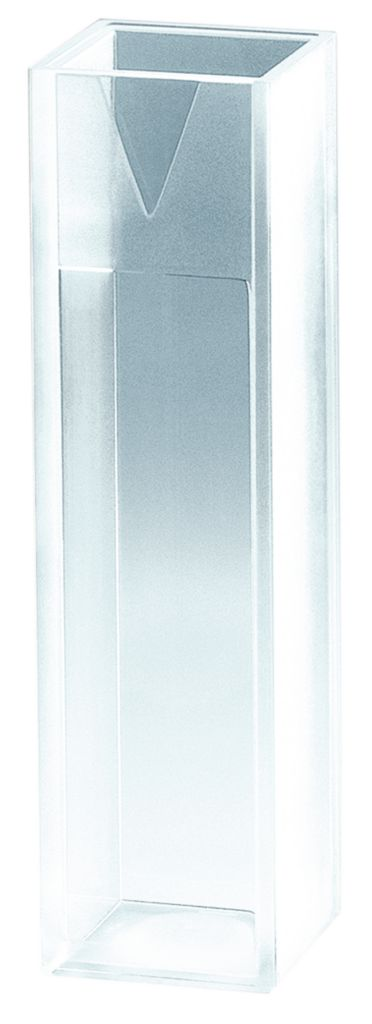
\includegraphics[scale=0.1]{PMMA_kyvett.jpg}
  \caption{PMMA-kyvett för engångsbruk}
  \end{center}
  \label{fig4}
\end{figure}

\subsection{Varför löser sig jod bättre i cyklohexanfasen?}

Läste att icke-polära lösningsmedel löser icke-polära föreningar vilket betyder att
Cyklohexan löser upp $\ch{I2}$. När detta skakas med $\ch{H2O}$ kan centeratomen som har negativ
formell laddning docka mot undersidan av spetsen hos vattenmolekylen.




\section{Spädning av en lösning}
Utrustning:\\
Om en milliliter används såsom startvolym för spädningen
\begin{enumerate}
\item 1 st automatpipett p1000\\
\item 1 st 10 ml bägare med 5 gånger 1 ml dvs. minst 6ml metylenblått\\
\item 2 st bägare 100 ml eller 1 st bägare 200 ml innehållande avjoniserat vatten
till egnalösningen med total vattenmängden minst\\
99+49+24+15+9=196ml. Tag 200ml

\item Bägare minst 35 ml med avjoniserat vatten till att späda provet.\\
Vattenmängd minst 9+9+9+2. Tag 35 ml.
\item 5 st bägare för att hålla 10ml, 16 ml, 25 ml, 50 ml och 100ml av egna lösningen
\item 5 st kyvetter till egna provet
\item 1 st mätcylinder 10 ml till utspädningen av provet
\item 1 st mätkolv 10 ml till utspädning av provet
\item 4 st bägare som som skall hålla minst 10ml av provet.
\item 4 st kyvetter till det utspädda provet.
\item 1 st Märkpenna
\end{enumerate}


Om man nu tar en given volym ur en lösning, låt oss säga 10,0 ml, ur en lösning som har
koncentrationen 0.5 M - hur många mol har man då? Enligt ekvationen ovan blir det 0,010 liter
multiplicerat med 0,5 mol/liter som blir 0,005 mol. Vi benämner denna volym och denna
koncentration med index 1.
\begin{flalign*}
n_1 &=c_1\cdot V_1\\
    &=0.5\cdot 0.010=0.005 \text{ mol}
\end{flalign*}
Om vi nu skulle späda de 10.0 ml upp till 100.0 ml, så finns det fortfarande 0.005 mol av ämnet -
men nu i 100.0 ml. Vi räknar ut koncentrationen:
\begin{flalign*}
n_2&=n_1\\
c_2&=\frac{n_1}{V_2}\\
    &=\frac{0.005}{0.1}=0.05\text{M}\\
\end{flalign*}


\subsection{Lambert-Beers lag}

När man vill kontrollera en koncentration för en lösning, kan man använda en kalibreringskurva. Det
förutsätter att det som finns i lösningen absorberar ljus, vid en given våglängd (som är olika för olika
ämnen). Om absorbansen är proportionell mot hur mycket som finns i lösningen (koncentrationen)
kan man konstruera en linjär kalibreringskurva.
\begin{flalign*}
A&=c\cdot l\cdot\epsilon\\
c&=\text{koncentration, [M]}\\
l&=\text{kyvettens bredd, [cm]}\\
\epsilon &=\text{molära absorptiviteten, }\Big[\frac{1}{\text{M}\cdot\text{cm}}\Big]\\
\end{flalign*}

\subsection{Förberedelser och spädning av lösningar}
Tilldelat är $0.15$mM metylenblått. 
Du ska tillreda 5 standardlösningar, genom att späda stamlösningen 100x, 50x, 25x, 16x samt 10x.

Antalet mol är det samma.
Utgå från 1 ml stamlösninglösning.
\begin{flalign*}
n_s&=c_s\cdot V_s\\
   &=0.15\cdot 10^{-3}\text{mol}\cdot\text{dm}^{-3}\cdot 0.001\text{dm}^{3}\\
   &=1.5000e-07\text{mol}
\end{flalign*}
Koncentration $c_1$ om man späder 10ggr är
\begin{flalign*}
c_1&=\frac{n_s}{10ml}\\
   &=\frac{1.5000e-07}{0.010}\\
   &=1.5000e-05\text{mol}= 0.015000\text{mM}
\end{flalign*}
Lämpligast tar man, 1 ml av stamlösningen och späder till
10ml, 16 ml, 25 ml, 50 ml och 100 ml.\\
Vilket betyder att avjoniserat vatten skall tillsättas med respektive
olika mängder.
$V_1=9$ ml, $V_2=15$ ml, $V_3=24$ ml, $V_4=50$ ml och $V_5=99$ ml om 1 ml stamlösning används.
\begin{flalign*}
V_{dissolve}=V_{origin}\cdot\text{times dissolve}-1
\end{flalign*}
Skript som beräknar spädningsvolymer och korresponderande koncentrationerna
och där förberedd anpassningsfunktion är placerad hittas på
\url{/home/lasse/Documents/Kurs/Inledande Kemi/Exercises/labb1_4.m}\\

Efter att koncentrationskurvan hittats tilldelas av läraren en okänt prov
som skall spädas på olika sätt.

\begin{enumerate}
\item späd 10x genom att använda mätcylinder till 10 ml slutvolym i en bägare.
Använd mätcylinder för att mäta upp 1 ml av den okända lösningen och fyll på med
9 ml avjoniserat vatten i mätcylindern slå sedan över till bägare.

\item Späd 10x genom att använda mätkolv till 10 ml slutvolym, använd automatpipett för att
tillsätta rätt volym av det okända provet.
\begin{figure}[H]
\begin{center}
  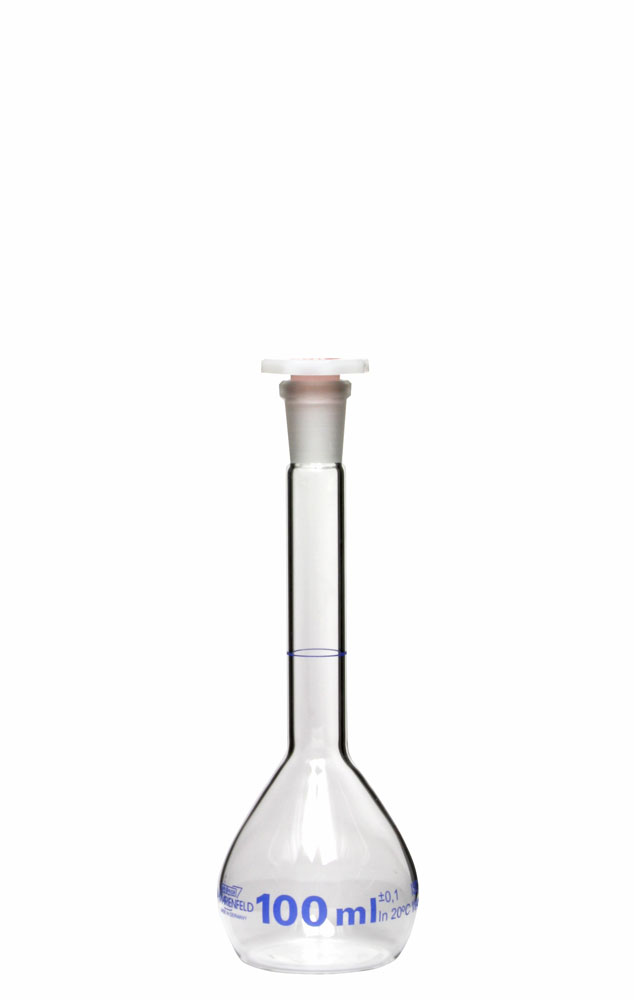
\includegraphics[scale=0.1]{mätkolv.jpg}
  \caption{Mätkolv}
  \end{center}
  \label{fig4}
\end{figure}
Ta upp 1 ml 1000 mikroliter med en p1000 automatpipett lägg i mätkolv. Fyll på med
avjoniserat vatten i mätkolven upp till 10 ml.

\item Späd 10x genom att använda automatpipett till slutvolymen 3 ml i en bägare.
Ta upp 3000/10= 300mikroliter med en p1000 pipett till förvaringsbägare.
Ta därefter med automat pippet upp 700mikroliter med p1000 automatpipett och
2* 1000 mikroliter med p1000 automatpipett

\item Späd 10x genom att använda bägare till 10 ml slutvolym, använd mätcylinder för att tillsätta
rätt volym av det okända provet.
Ta upp 1 ml med mätcylinder. Fyll på med 9 ml i bägaren användandes av bägarens volymsstreck.
\end{enumerate}
\subsection{Absorbansmätningar}

Absorbans skall mätas för alla prov och standardlösningar en spektrofotometer vid våglängden
665nm, enligt handledarens instruktion. Var noga med att skriva upp alla uppmätta värden i din
labbok. Använd avjoniserat vatten som referens och PMMA kyvetter.

\newpage

%\vfill\null
%\clearpage
%\columnbreak
%\newpage



%\underbrace{}

% \hspace{1em}

%\begin{enumerate}[label=(\alph*)]
%\end{enumerate}

%$$
%  A = 
%  \begin{bmatrix}
%    1 & 0  & 2i\\
%    2i & 0 &  -4\\
%    -i &  0 & -2i\\
%  \end{bmatrix}
%$$

%\begin{flalign*}
%  A = 
%  \begin{bmatrix}
%    1 & 0  & 2i\\
%    2i & 0 &  -4\\
%    -i &  0 & -2i\\
%  \end{bmatrix}
%\end{flalign*}


%\begin{flalign*}
%\psi(x) = \begin{cases} Ae^{ikx}+Be^{-ikx} &\ \  x<-a \\
%                        Ce^{\kappa x}+De^{-\kappa x} &\ \ -a < x < a\\
%						Fe^{ikx} & \ \ x>a
%       \end{cases}
%\end{flalign*}

%\begin{figure}[H]
%  \includegraphics[width=\linewidth]{odd_finite.eps}
%  \caption{$z_0=0.1\pi,0.5\pi, 3\pi,7\pi$}
%  \label{fig4}
%\end{figure}
\end{document}








\vfill\null
\clearpage
\columnbreak
\newpage










                                     
                                     



